\documentclass[00_doc.tex]{subfiles}
\begin{document}
    \subsection{Ideas}
    \subsubsection{Color-changing Bracelet}
    \begin{flushleft}
        Our first idea was to program and color-changing bracelet. This can change its color if someone of your
        friends has such a bracelet too. These can create a network, so they can communicate with each other. The
        network strength can be used to identify if the friend is close. Then it will change its color, so both know
        that a friend is close to him or her. Also, groups can be defined. Every group has its own thread and if someone 
        from a specific group is next to you the system can change the color of this specific thread. This would just 
        be a proof of concept, so most of the programming would be static (see Figure ~\ref{fig:braceltIdea}).
    \end{flushleft}

    \begin{figure}[h!]
        \centering
        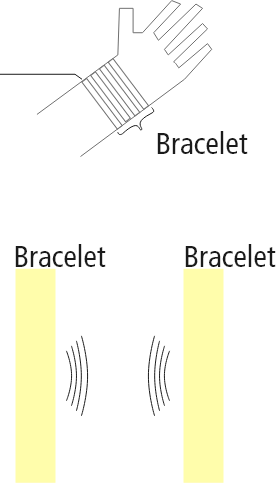
\includegraphics[scale=0.4]{images/projectideas/bracelt.png}
        \caption{Shows the bracelt concept.}
        \label{fig:braceltIdea}
    \end{figure}

    \subsubsection{Music controll Jacket}
    \begin{flushleft}
        Another idea was to develop a jacket that can be used to change a song you are listening on a phone. Therefore,
        strips are placed on the left or right arm that can be used to change the song to make it louder or to stop the song, 
        for example (see Figure ~\ref{fig:jacketIdea}).
    \end{flushleft}

    \begin{figure}[h!]
        \centering
        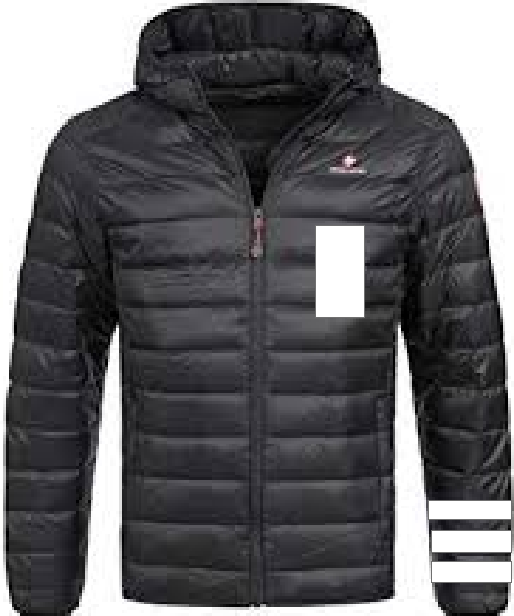
\includegraphics[scale=0.2]{images/projectideas/jacket.png}
        \caption{Shows the concept of a jacket with interaction constraints.}
        \label{fig:jacketIdea}
    \end{figure}

    %why is the new chapter before image? 
    \subsubsection{Blossom shaped Lamp}
    \label{BlossomShapedLamp}
    \begin{flushleft}
        A third and last idea is about lightness. The idea is to build a lamp of a blossom that can be modified by the user.
        Every blossom leaf has a magnet inside, so it is possible to connect each leave. If some leaves are connected, the lamp that 
        is in the middle of the flower blossom changes its color. Moreover, it is possible to rotate the whole lamp and to change the
        brightness by an analog switch (see Figure ~\ref{fig:blossomLamp}).
    \end{flushleft}

    \begin{figure}[h!]
        \centering
        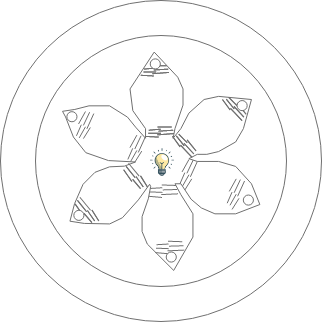
\includegraphics[scale=0.4]{images/projectideas/blossomLamp.png}
        \caption{Shows the concept of a blossom shaped lamp.}
        \label{fig:blossomLamp}
    \end{figure}
\end{document}